\documentclass[aspectratio=169,10pt]{beamer}
\usetheme{Boadilla}
\usepackage{graphicx,booktabs}
\title{One-photon pseudoscalar feed-down in the v3 analysis}
\subtitle{100k physics-model events per mode; frozen 1,091-chunk BDT proposal}
\author{FCC-ee $\Lambda_b\to\Lambda\gamma$ analysis}
\date{4 October 2026}
\begin{document}
\frame{\titlepage}
\begin{frame}{Question and exact comparison}
\begin{itemize}
\item Forced $\Lambda_b\to\Lambda\eta(\gamma\gamma)$ and $\Lambda_b\to\Lambda\pi^0(\gamma\gamma)$ HELAMP samples; both charge conjugates, 100,000 input events each.
\item Same one-photon Stage 1 v3 builder, $\Lambda$ mass $\pm12.5$ MeV, $E_{\Lambda_b}\geq10.5$ GeV, same hemisphere, no meson veto.
\item Validation-fixed BDT score $\geq0.9538269639$; physical estimates use candidate rows in a provisional $5.4$--$5.9$ GeV reconstructed signal window.
\item Truth ancestry labels direct partial and wrong combinations after reconstruction and selection.
\end{itemize}
\end{frame}
\begin{frame}{Generated model checks}
\centering
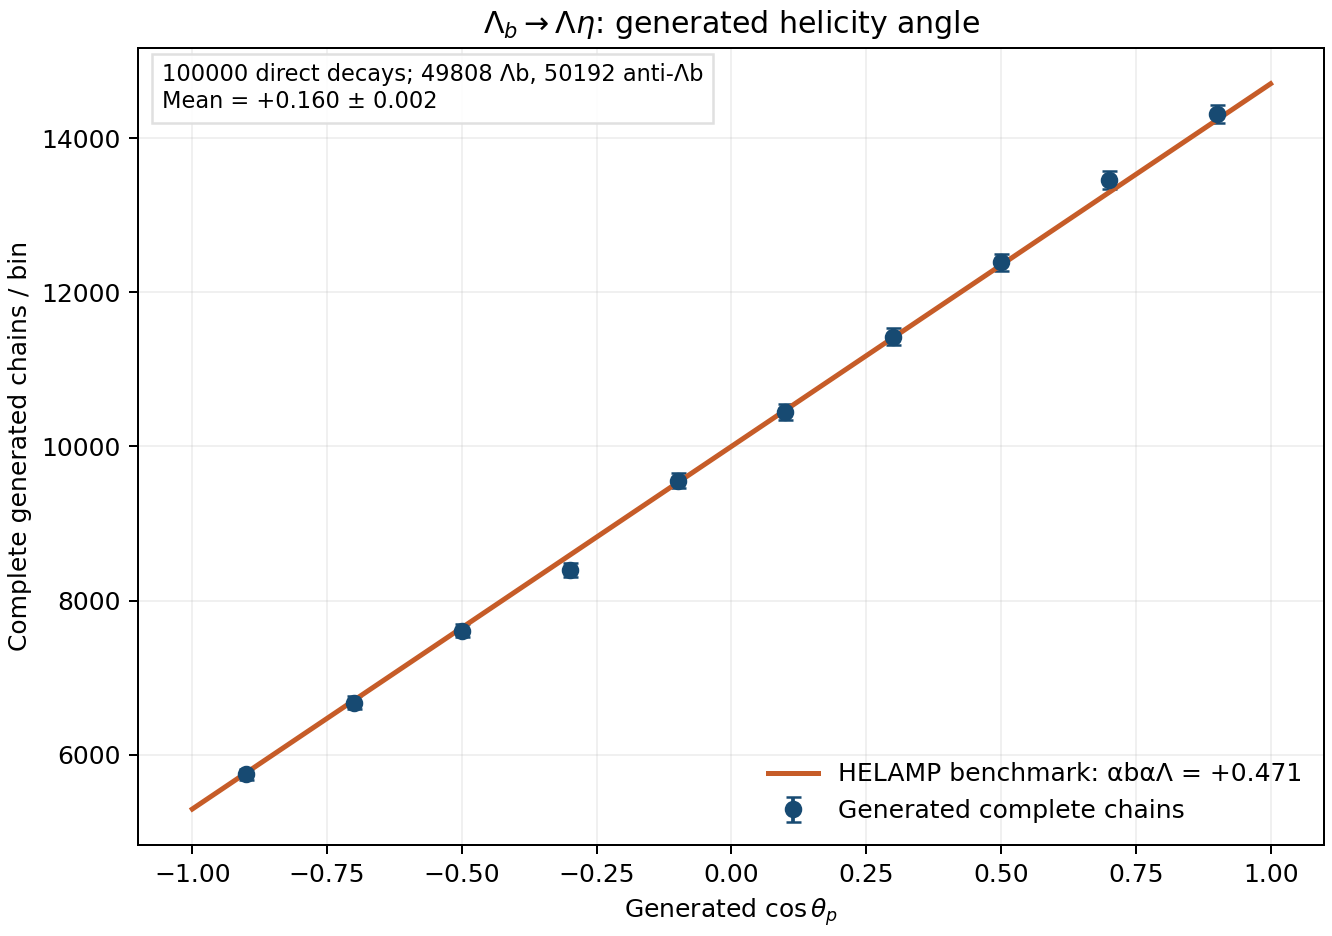
\includegraphics[width=.48\textwidth]{figures/eta_physics_generated_angle.png}\hfill
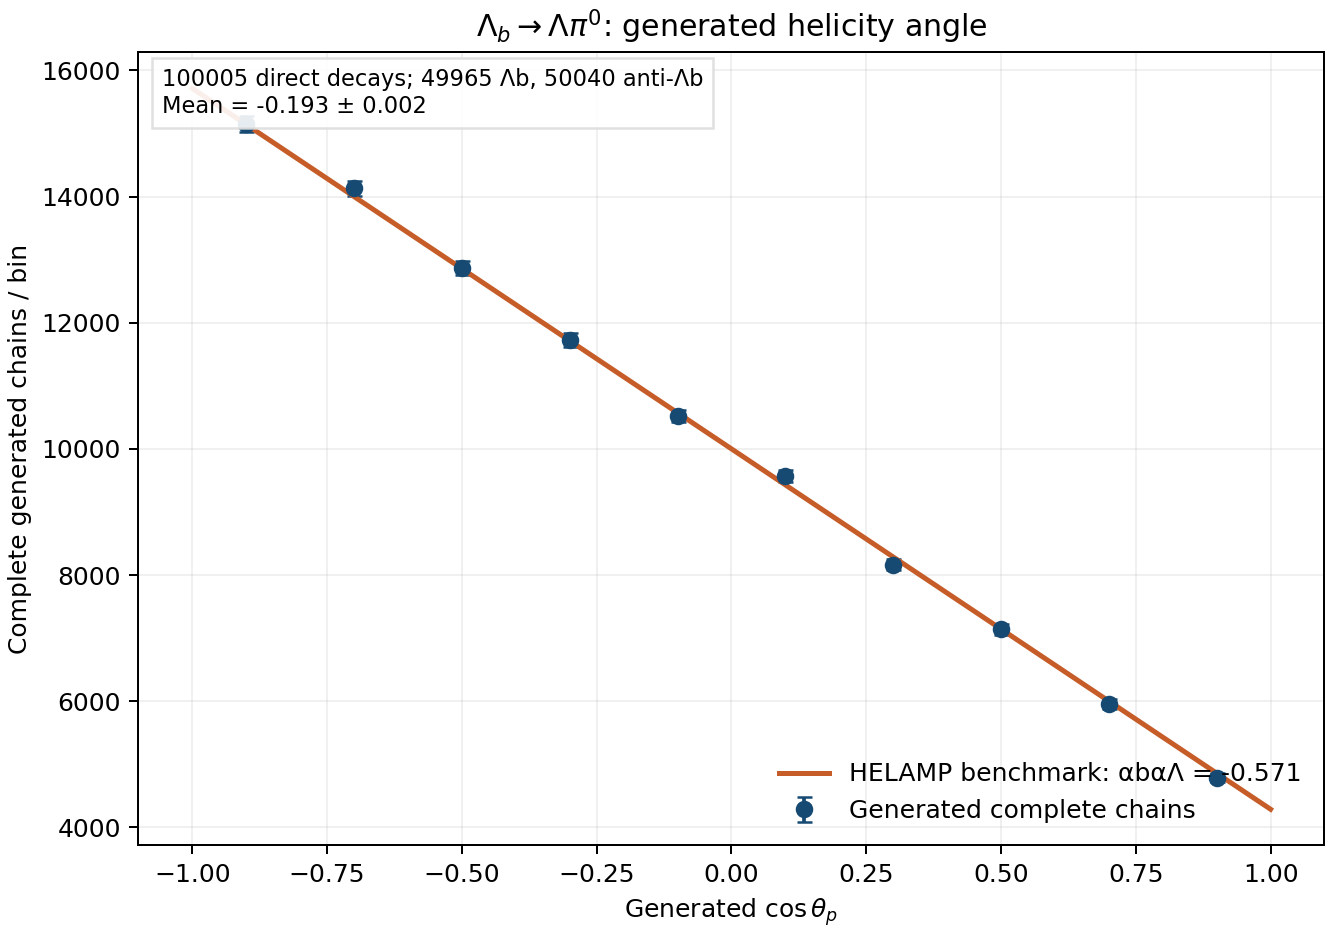
\includegraphics[width=.48\textwidth]{figures/pi0_physics_generated_angle.png}
\end{frame}
\begin{frame}{Stage-by-stage reconstructed mass}
\centering
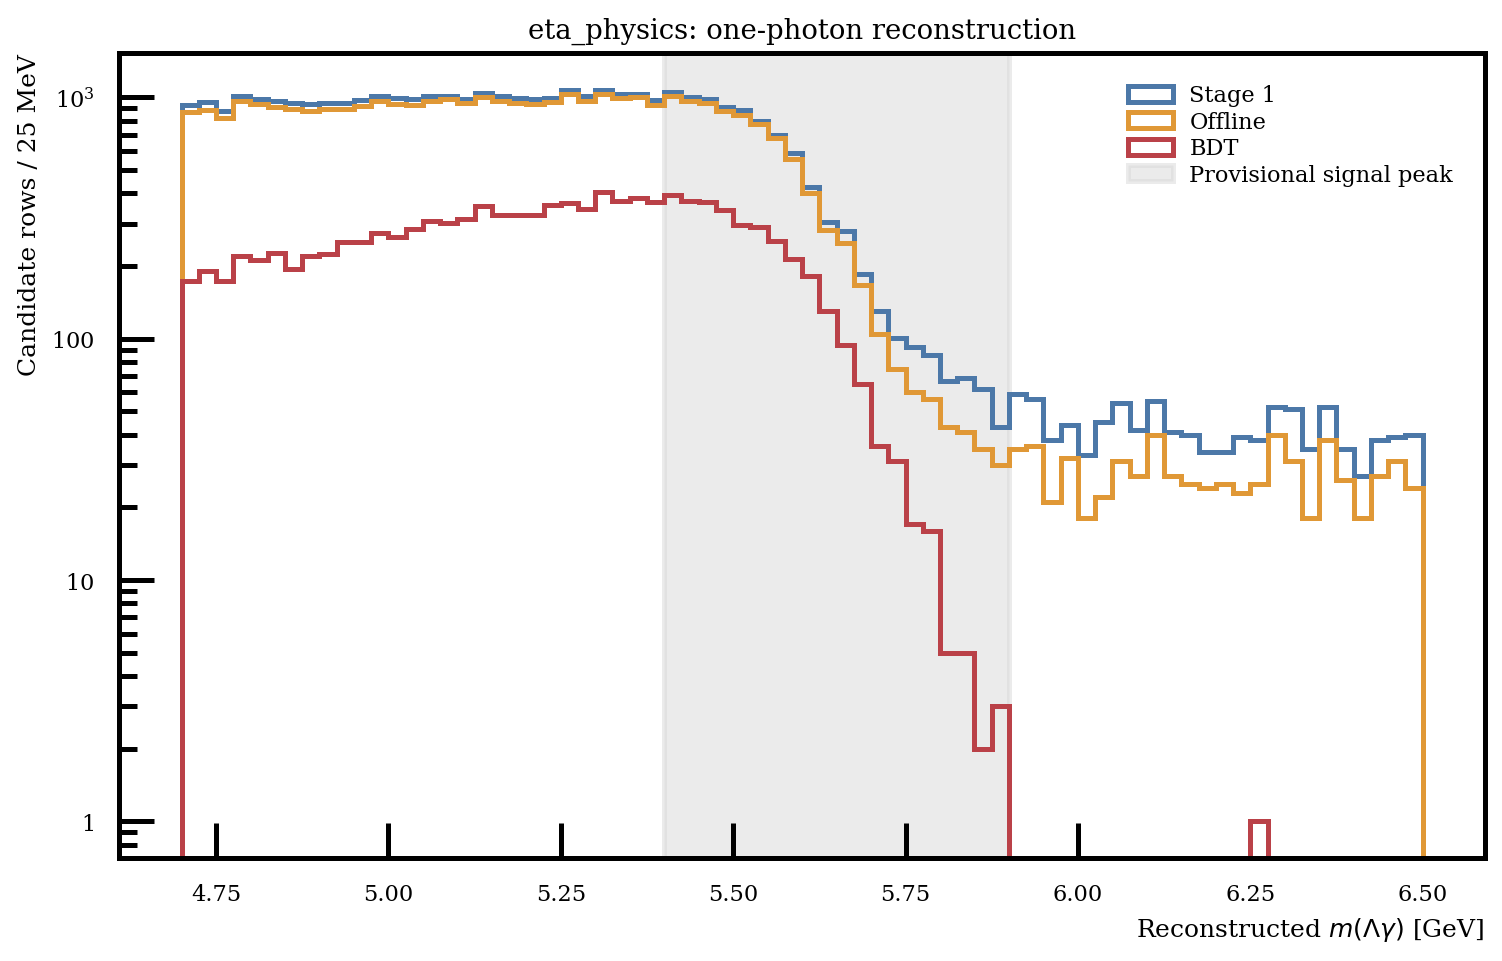
\includegraphics[width=.48\textwidth]{figures/eta_physics_mass_cutflow.png}\hfill
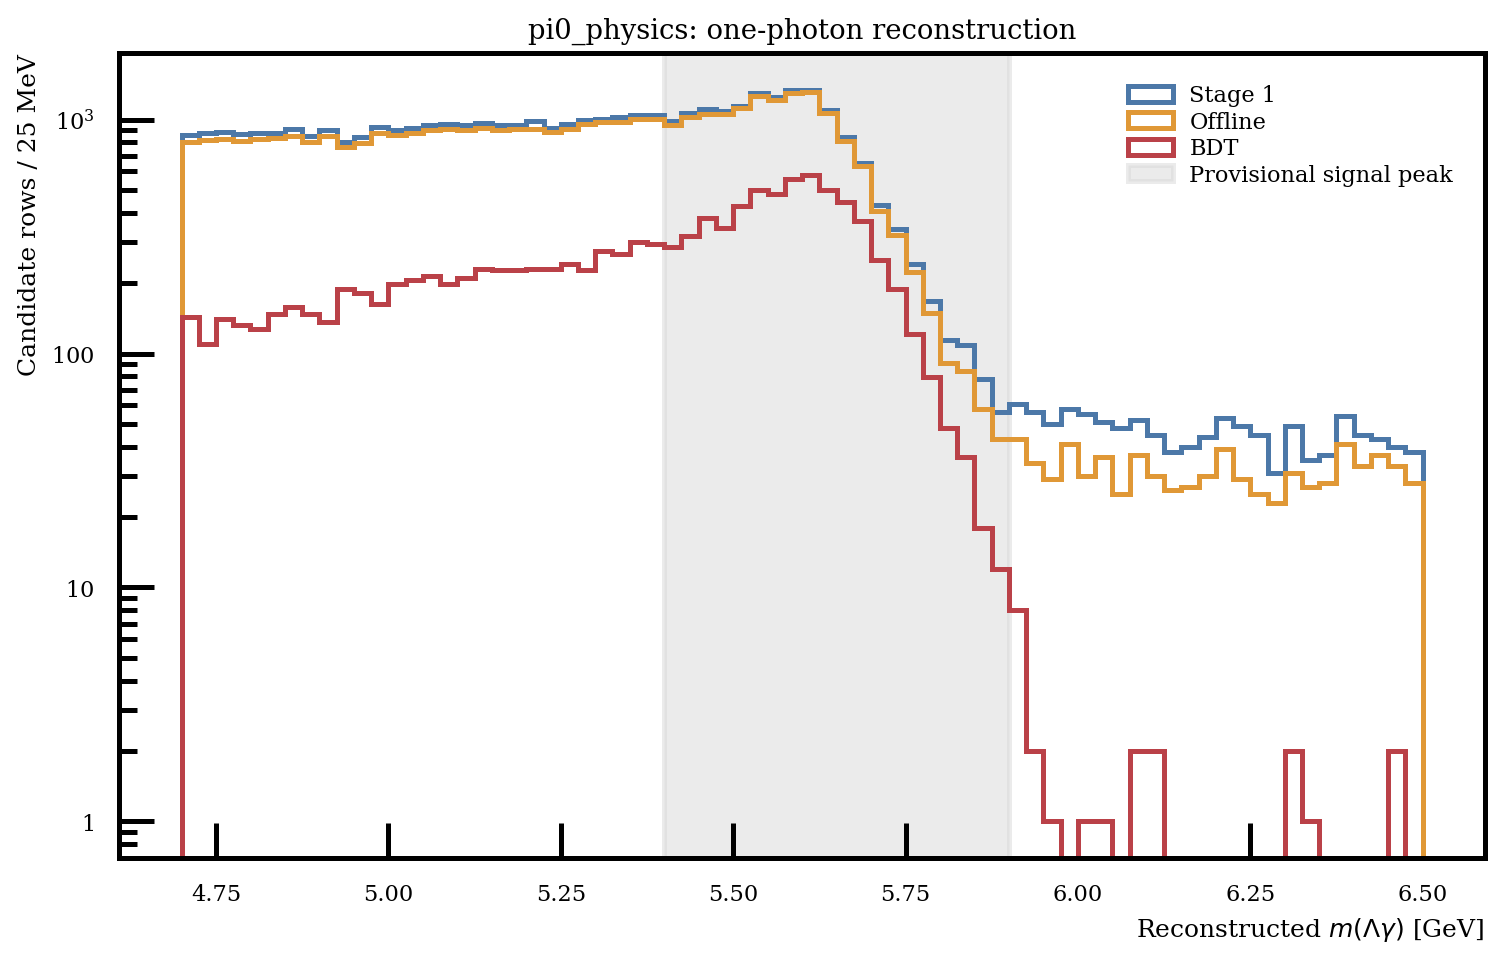
\includegraphics[width=.48\textwidth]{figures/pi0_physics_mass_cutflow.png}
\end{frame}
\begin{frame}{Surviving ancestry and angular shape}
\centering
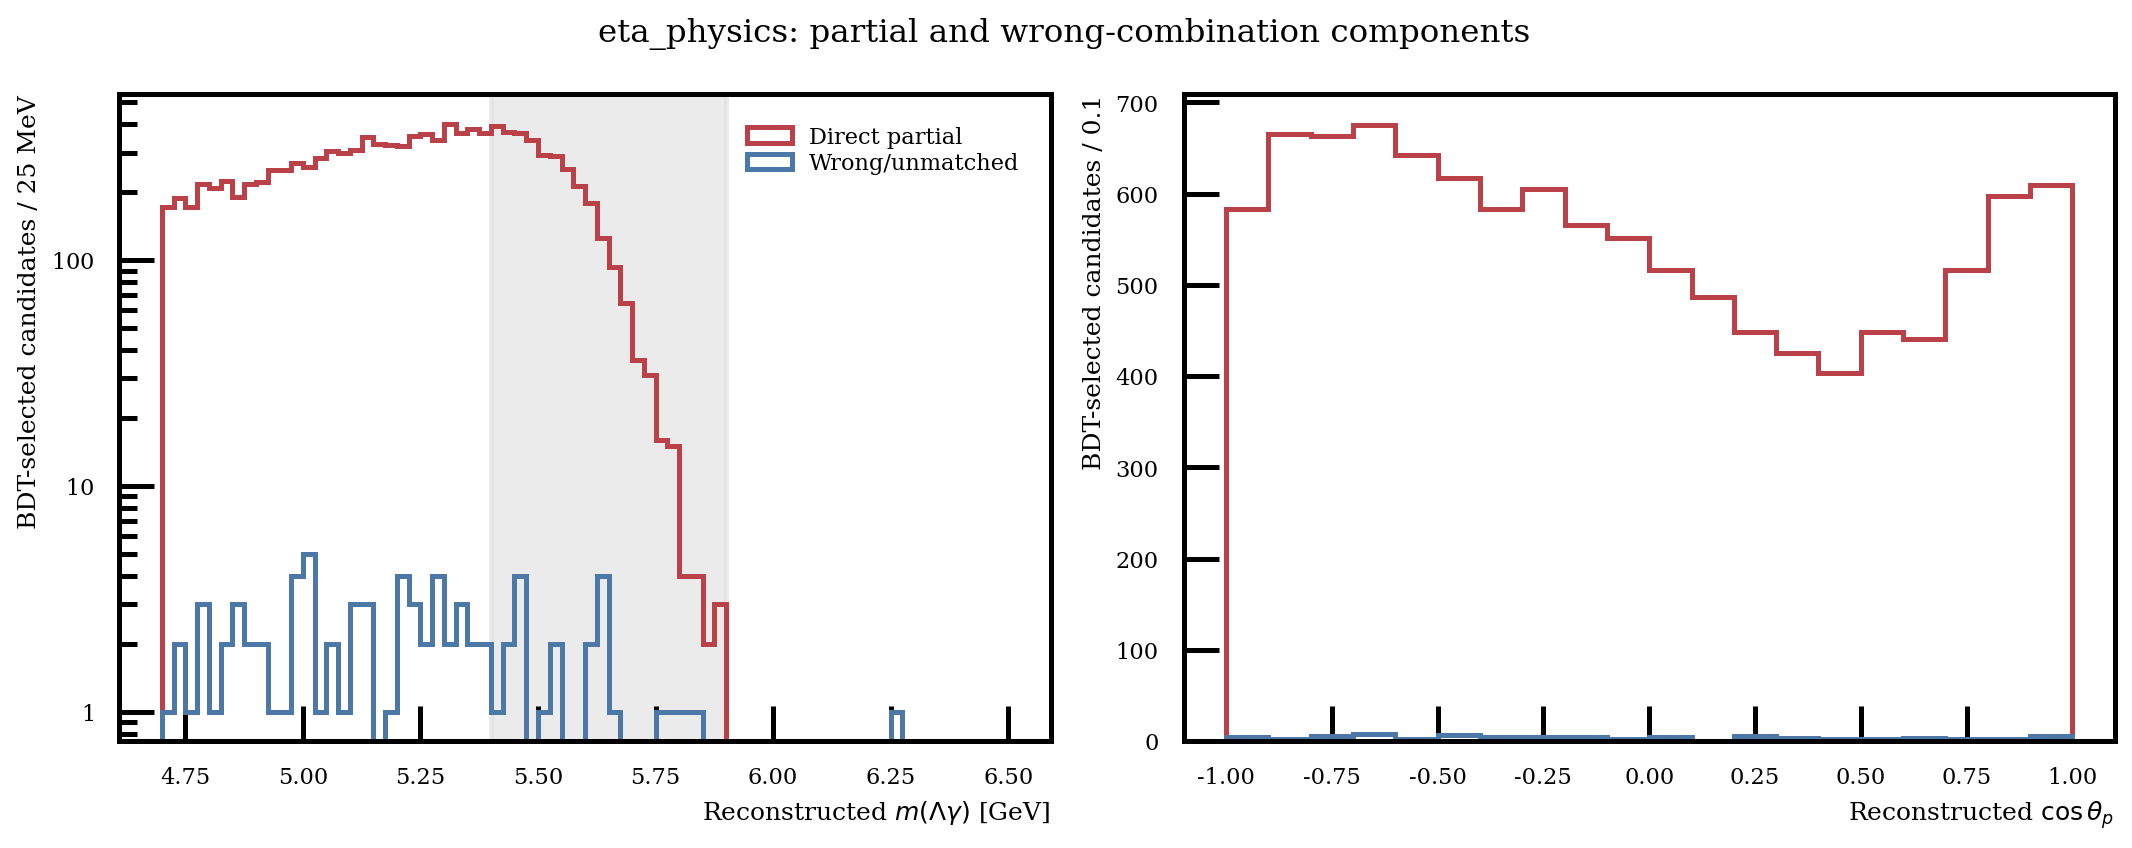
\includegraphics[width=.48\textwidth]{figures/eta_physics_post_bdt_mass_angle.png}\hfill
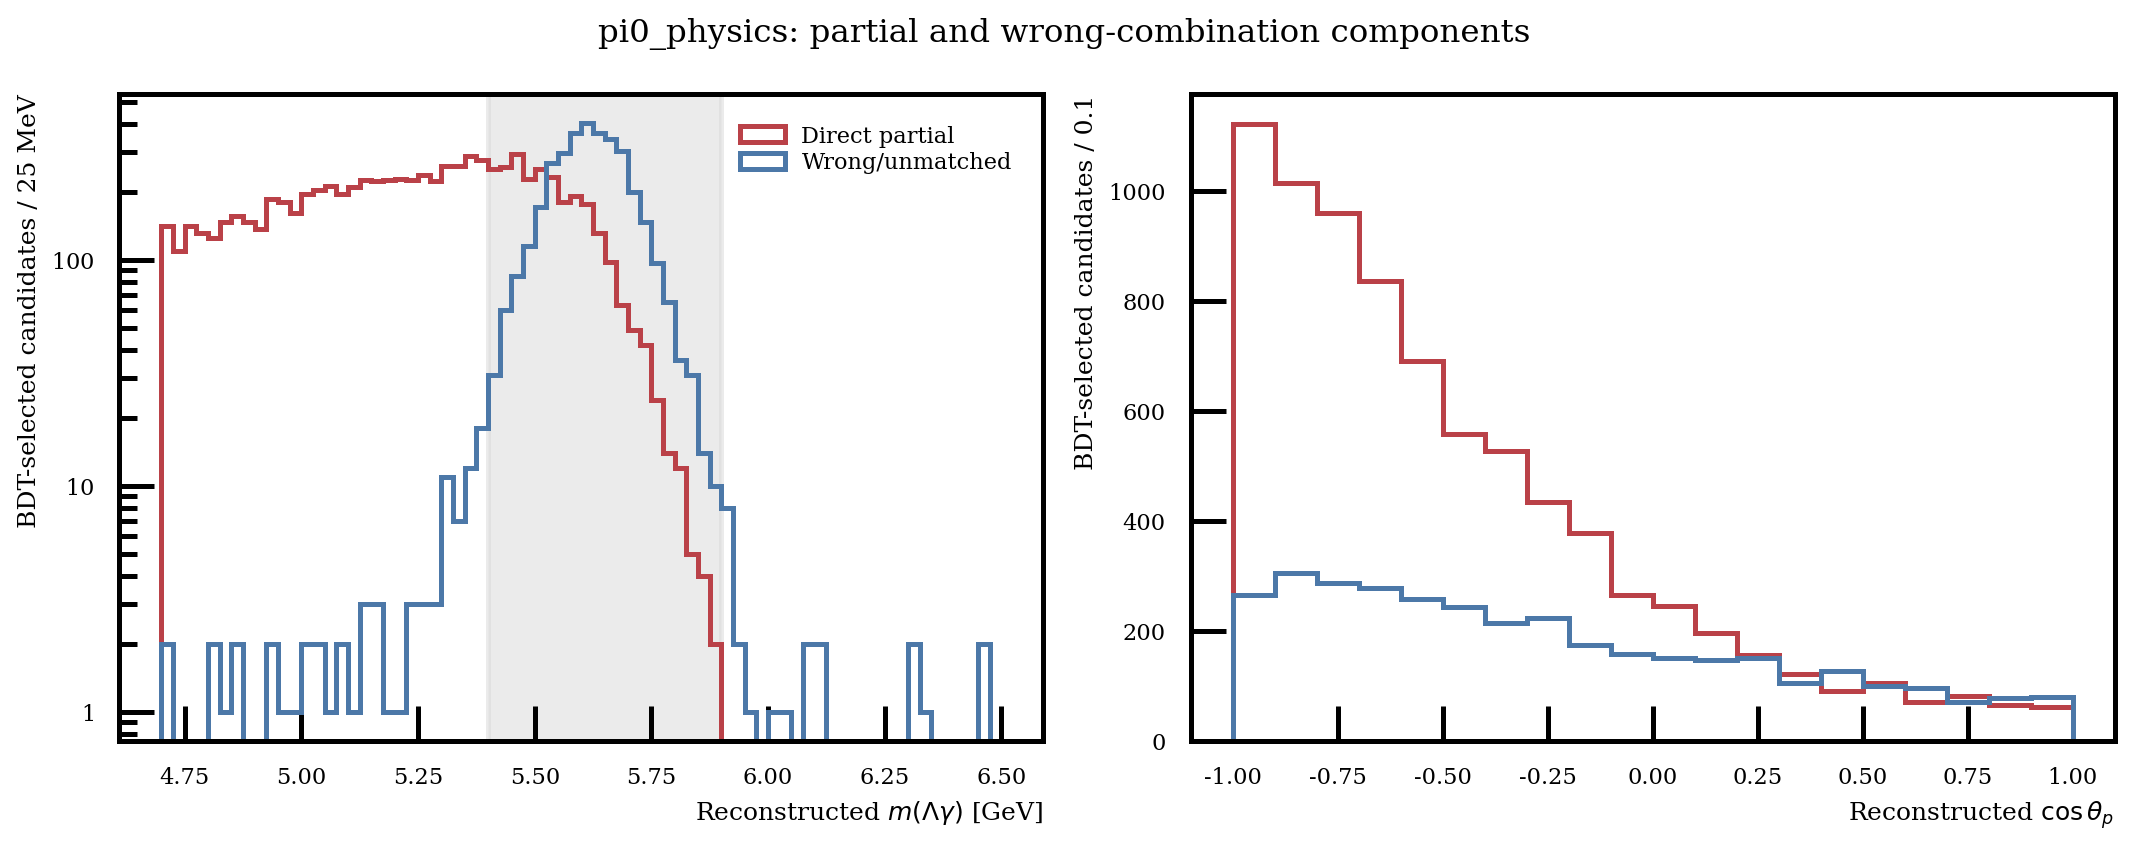
\includegraphics[width=.48\textwidth]{figures/pi0_physics_post_bdt_mass_angle.png}
\end{frame}
\begin{frame}{Candidate counts and denominators}
\small
\begin{tabular}{lrr}
\toprule
Quantity & $\Lambda\eta$ & $\Lambda\pi^0$\\
\midrule
Generated direct decays & 100,000 & 100,005\\
Stage 1 candidate-bearing events & 41,752 & 45,104\\
Stage 1 candidate rows & 44,717 & 48,298\\
Offline candidate rows & 35,267 & 39,639\\
BDT candidate rows & 11,125 & 11,512\\
Peak candidate rows & 3,120 & 5,937\\
Peak direct partial / wrong rows & 3,099 / 21 & 2,519 / 3,418\\
\bottomrule
\end{tabular}
\vspace{.7em}

Offline retention from Stage 1: 78.87\% / 82.07\%. BDT retention from offline: 31.55\% / 29.04\%. These are forced-sample candidate rates, before branching normalization.
\end{frame}
\begin{frame}{Physical scenarios, shown separately from inclusive $Z\to b\bar b$}
\centering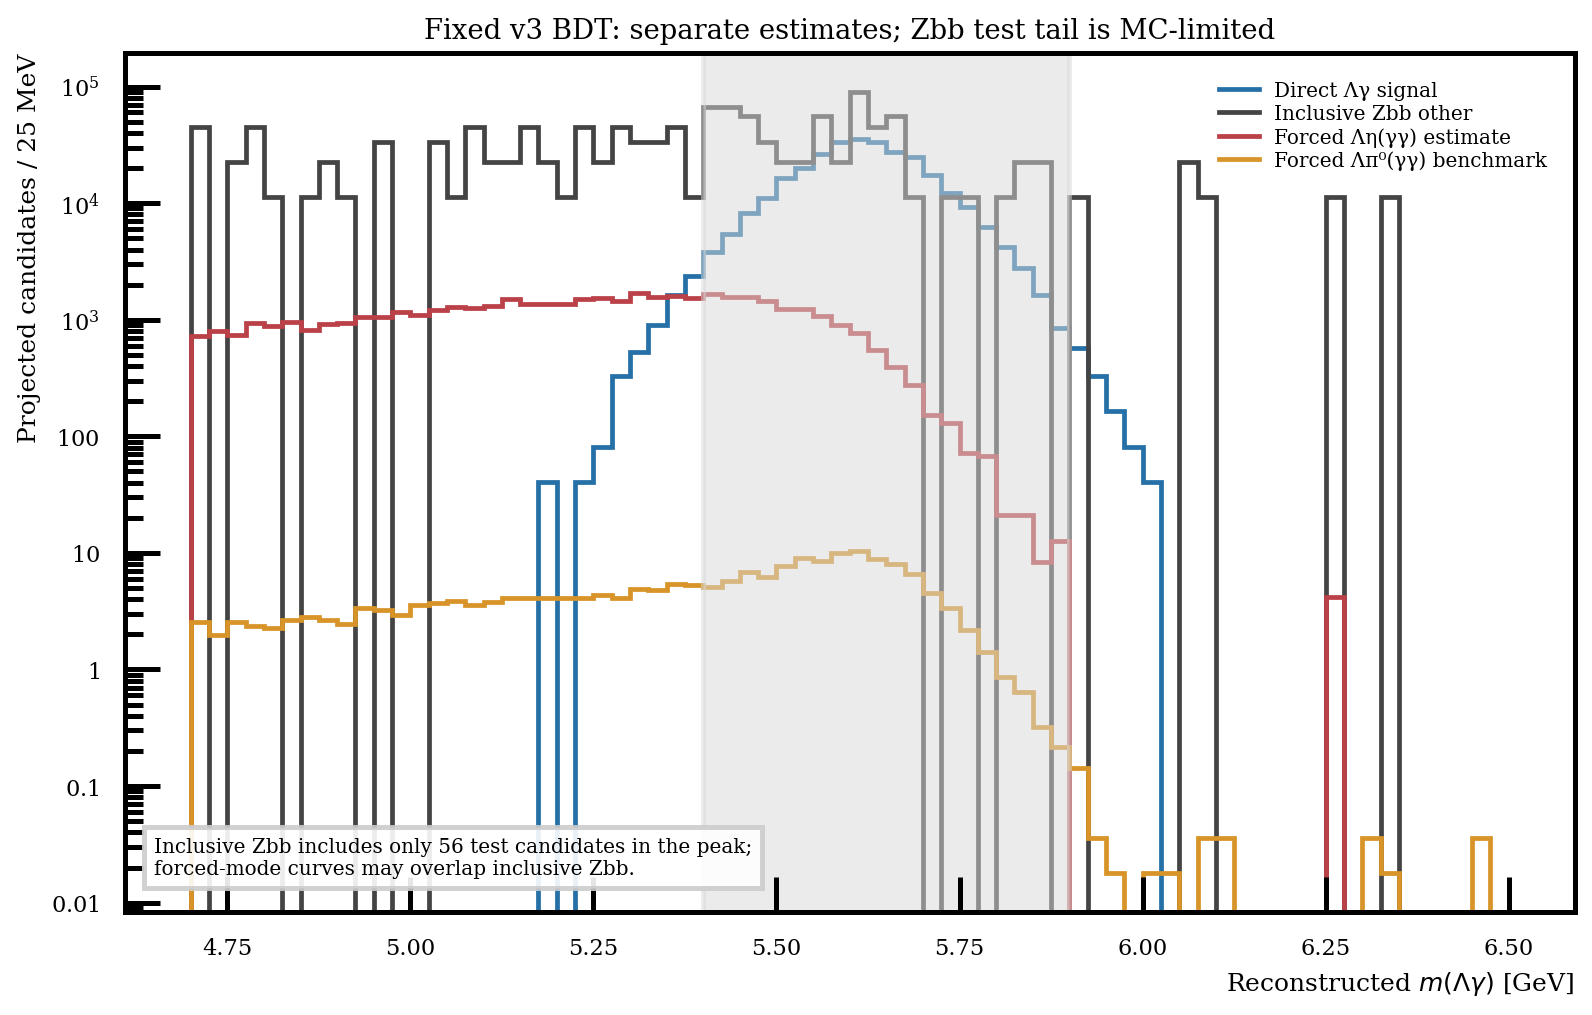
\includegraphics[height=.77\textheight]{figures/expected_mass_comparison.png}
\end{frame}
\begin{frame}{Interpretation and PI decision}
\begin{itemize}
\item With $N_Z=6\times10^{12}$ and stated production and daughter fractions: $\Lambda\eta$ contributes about 13,136 peak candidates using the LHCb parent-BR central value; $\Lambda\pi^0$ contributes about 107 using a theory parent-BR benchmark.
\item At fixed branching inputs, approximate candidate-count MC 95\% intervals: 12,679--13,605 and 104--109. Parent-BR uncertainty dominates the $\eta$ estimate; $\pi^0$ has no measured parent input here.
\item Inclusive $Z\to b\bar b$ can already contain these modes. Audit overlap before adding forced-mode estimates to it. The inclusive peak shape has only 56 held-out test candidates.
\item Decide whether to include explicit feed-down shapes and adopt a peak window and branching scenarios; the BDT score remains a proposal.
\end{itemize}
\end{frame}
\end{document}
